\section{Motivational Experiments}
\label{experiment}


In literature, we find only two modularity definitions for multlayer networks - one by Liu et al. in~\cite{CompMod} and the other 
by Song et al. in~\cite{medical_paper}. We have already discussed the limitations of the definition proposed in~\cite{CompMod}
in Sec.~\ref{intro}.
In this section, we criticize the metric proposed in~\cite{medical_paper} with the help of different synthetic network
configurations and emphasize on the need of proposing a new modularity metric for generic multilayer networks.

% As we mentioned before, some of the existing methods only find multilayer communities and some of them only find single layer communities.
% The algorithm proposed in \cite{medical_paper} seems to be our closest competitor at present. So, in the following we criticize the modularity
% metric they proposed.
For a 2-layer (suppose, A and B) network $G=G_A \cup G_\pi \cup G_B$ where $G_A$ = ($V_A$, $E_{AA}$) is the subnetwork 
of class A, $G_B$ =
($V_B$, $E_{BB}$) is the subnetwork of class B, and $G_\pi$ = ($V_A$, $V_B$, $E_{AB}$) is a bipartite graph connecting
nodes of class A and class B, the modularity metric proposed in \cite{medical_paper} is defined as 
\begin{equation}\label{eqn1}
 mQ=\frac{1}{3}\sum_{c=1}^{n_c}\{[\frac{I_{Ac}}{m_A}-(\frac{d_{Ac}}{2m_A})^2]+[\frac{I_{\pi c}}{m_\pi}-\frac{k_{\pi c}\times{d_{\pi c}}}{{m_\pi}^2}]+
 [\frac{I_{Bc}}{m_B}-(\frac{d_{Bc}}{2m_B})^2]\}
\end{equation}
where $n_c$ is the number of modules in a given partition; each module c is virtually divided into three
submodules, c = $(Ac)\cup(\pi c)\cup(Bc)$, $Ac$ is the submodule with links from $E_{AA}$, $\pi c$ is from $E_{AB}$
and $Bc$ is from $E_{BB}$; $I_{Ac}$ is the number of links in submodule $Ac$, $m_A$ is the size of subnetwork
$G_A$, $d_{Ac}$ is the sum of degrees of all $Ac$ nodes in $G_A$; $k_{\pi c}$ is the sum of degrees of A nodes of $\pi c$
in subnetwork $G_\pi$, $d_{\pi c}$ is the sum of degrees of B nodes of $\pi c$ in $G_\pi$.
In fact, this definition is basically a linear combination of Newman-Girvan modularity for simple graph~\cite{newman2004finding} 
and Barber modularity for bipartite graph~\cite{barber2007modularity}.

\begin{figure}
\centering
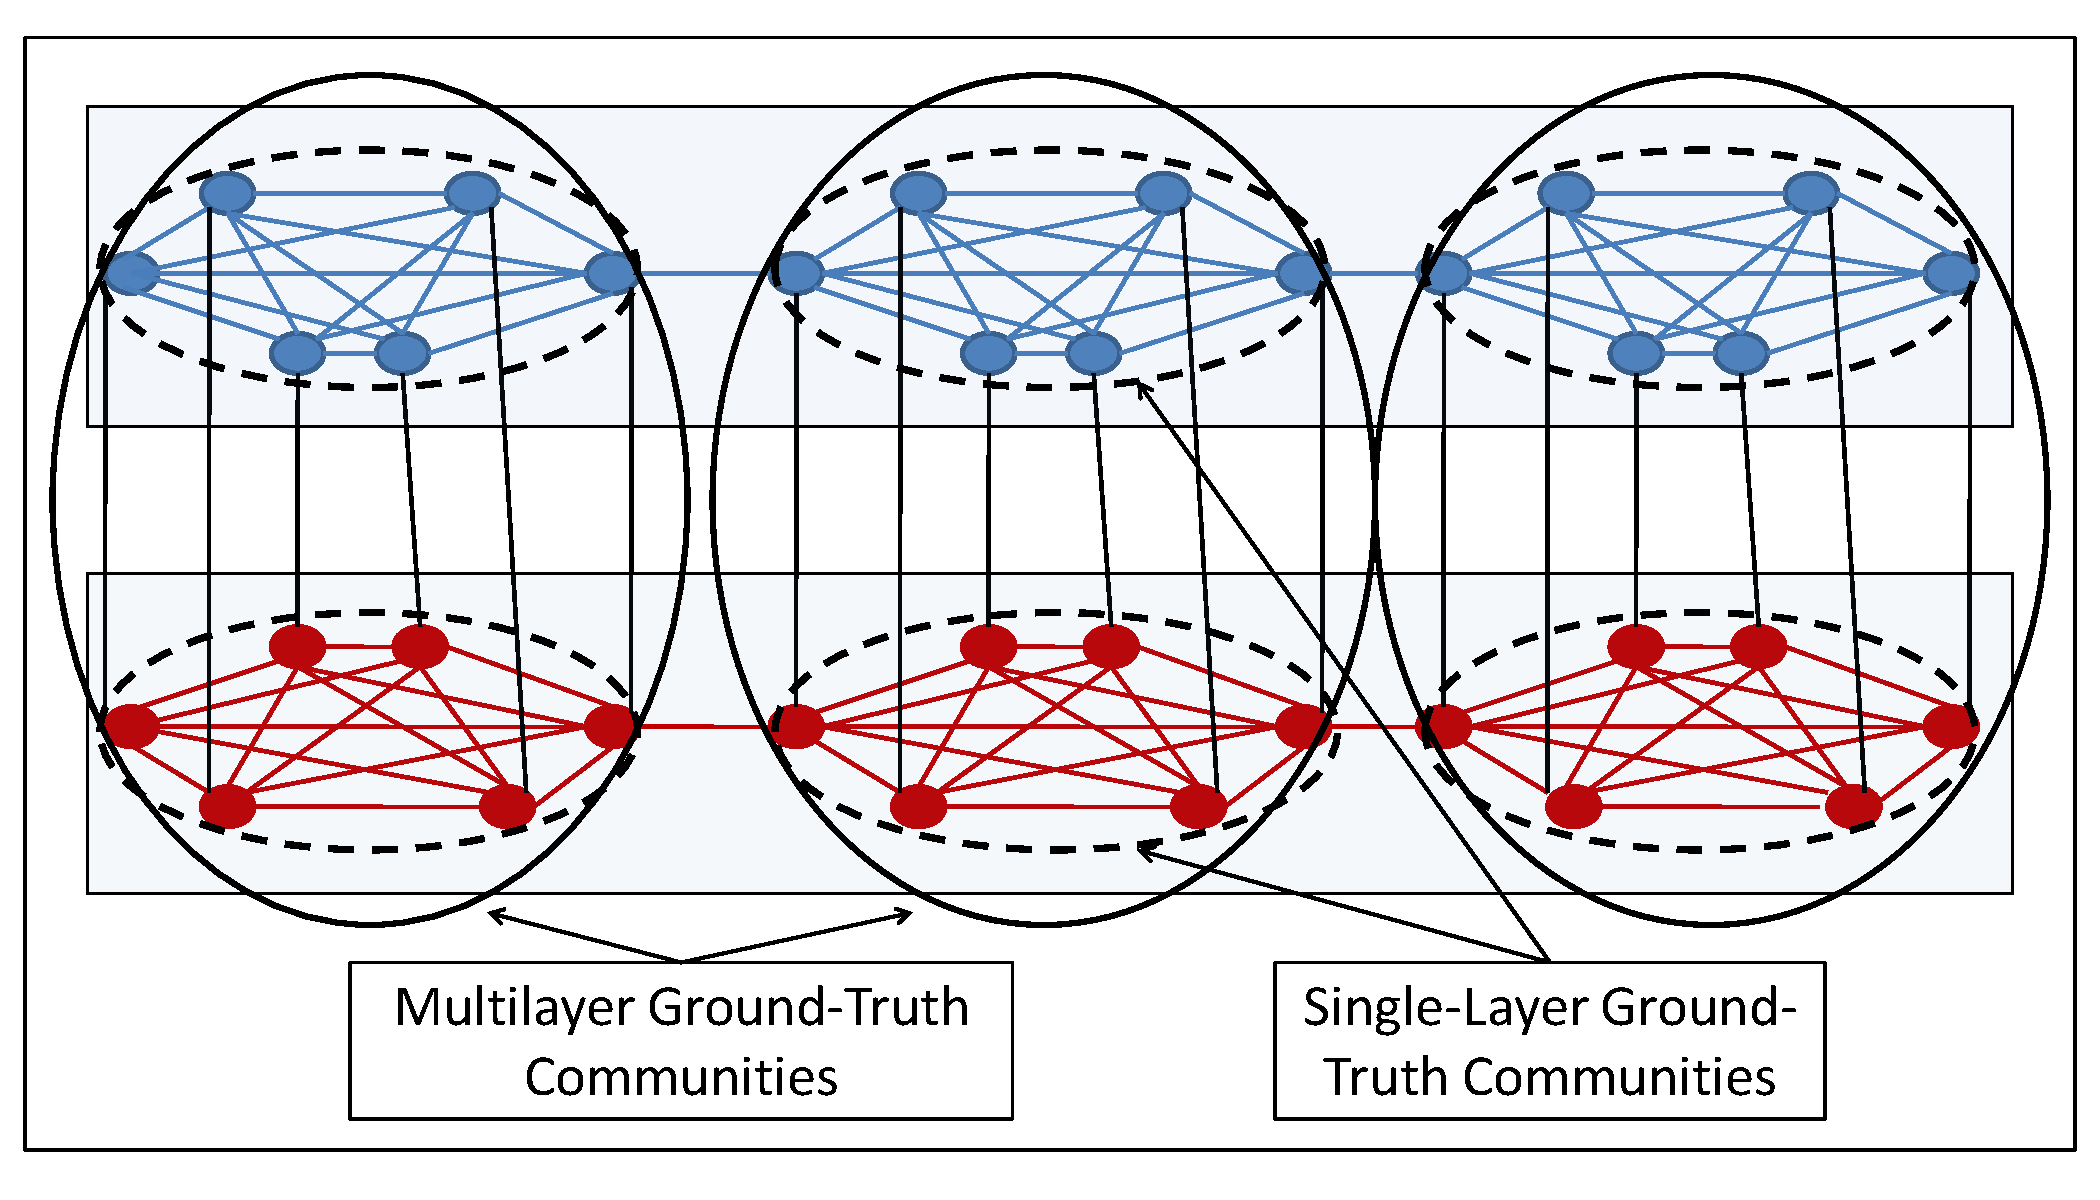
\includegraphics[width=3.5in]{./images/motivation.pdf}
\vspace{-0.1in}
\caption{Network configuration with two different ground truth communities}
\vspace{-0.1in}
\label{N0}
\end{figure}

% \begin{figure}
% \begin{center}
% \subfigure[Starting Configuration
% ]{\label{NN0}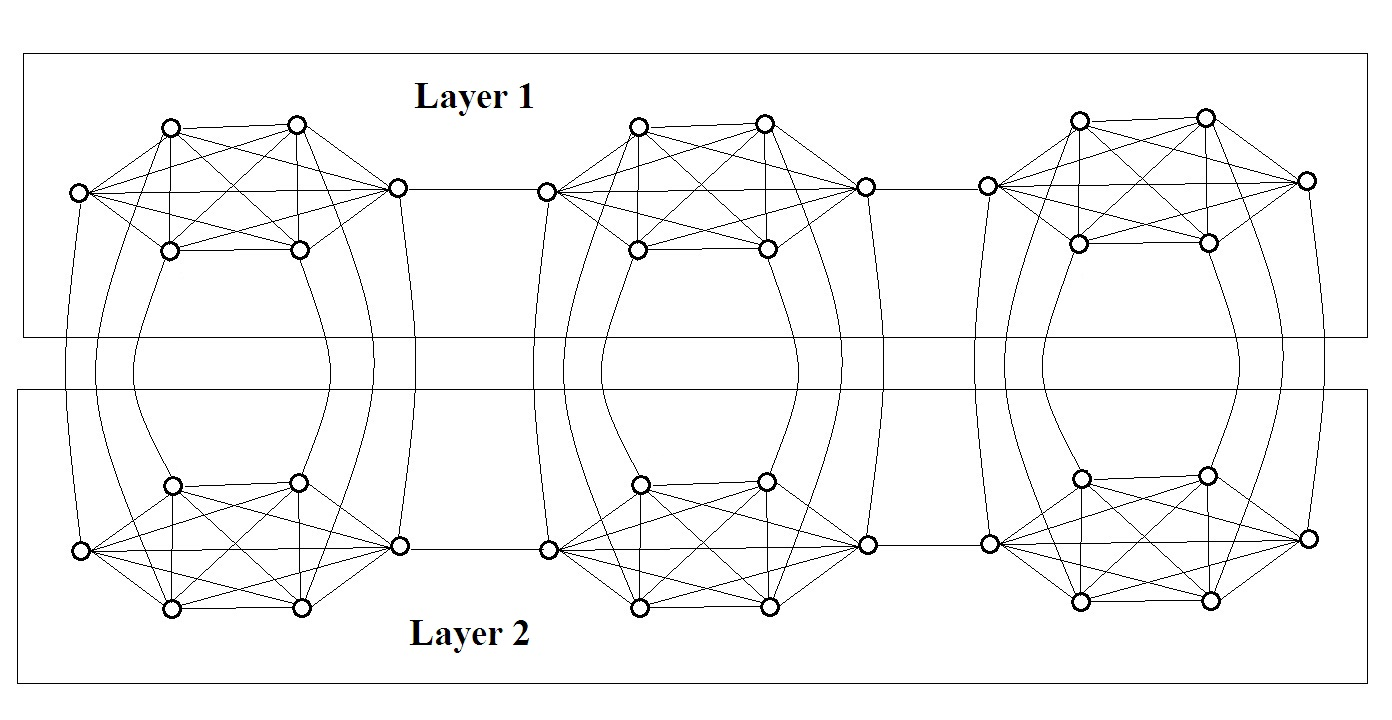
\includegraphics[angle=0,scale=.25]{./images/network0.jpg}}
% \subfigure[Ground Truth multilayer communities
% ]{\label{N01}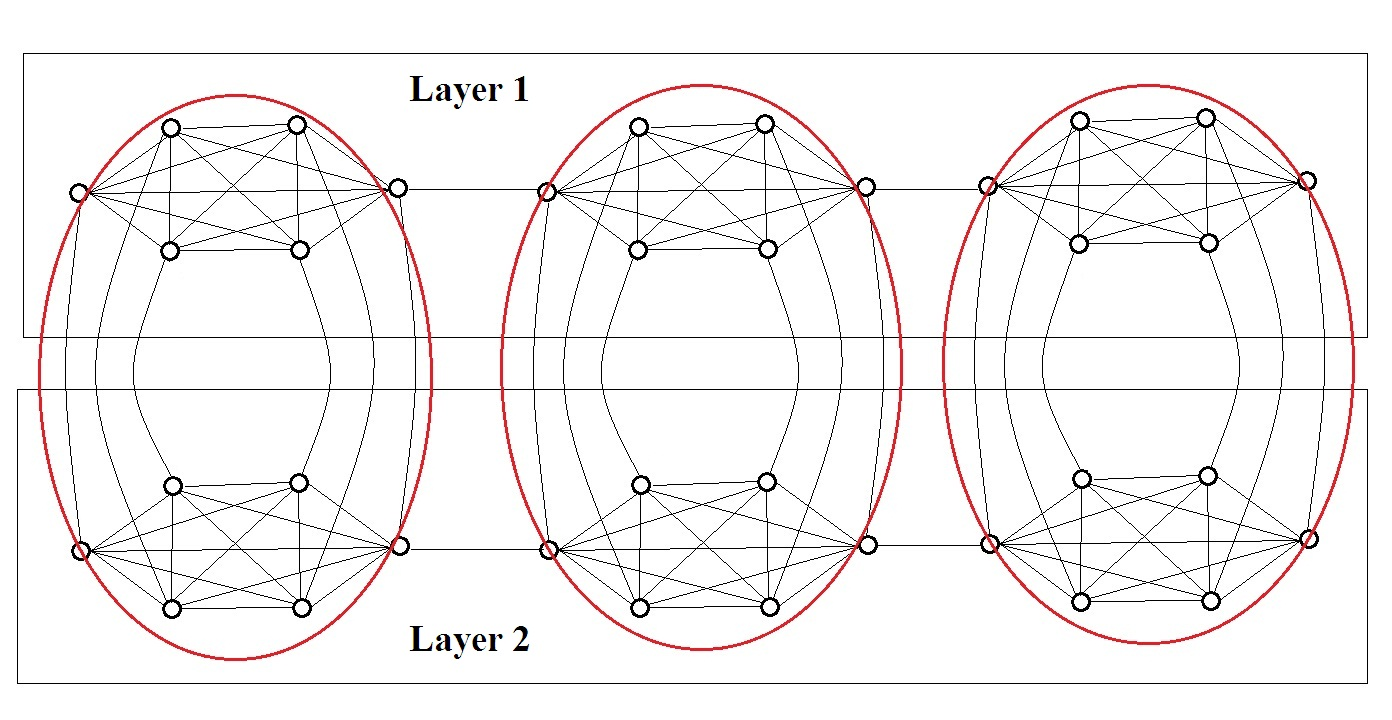
\includegraphics[angle=0,scale=.25]{./images/network0_1.jpg}}
% \subfigure[Ground Truth Single layer communities
% ]{\label{N02}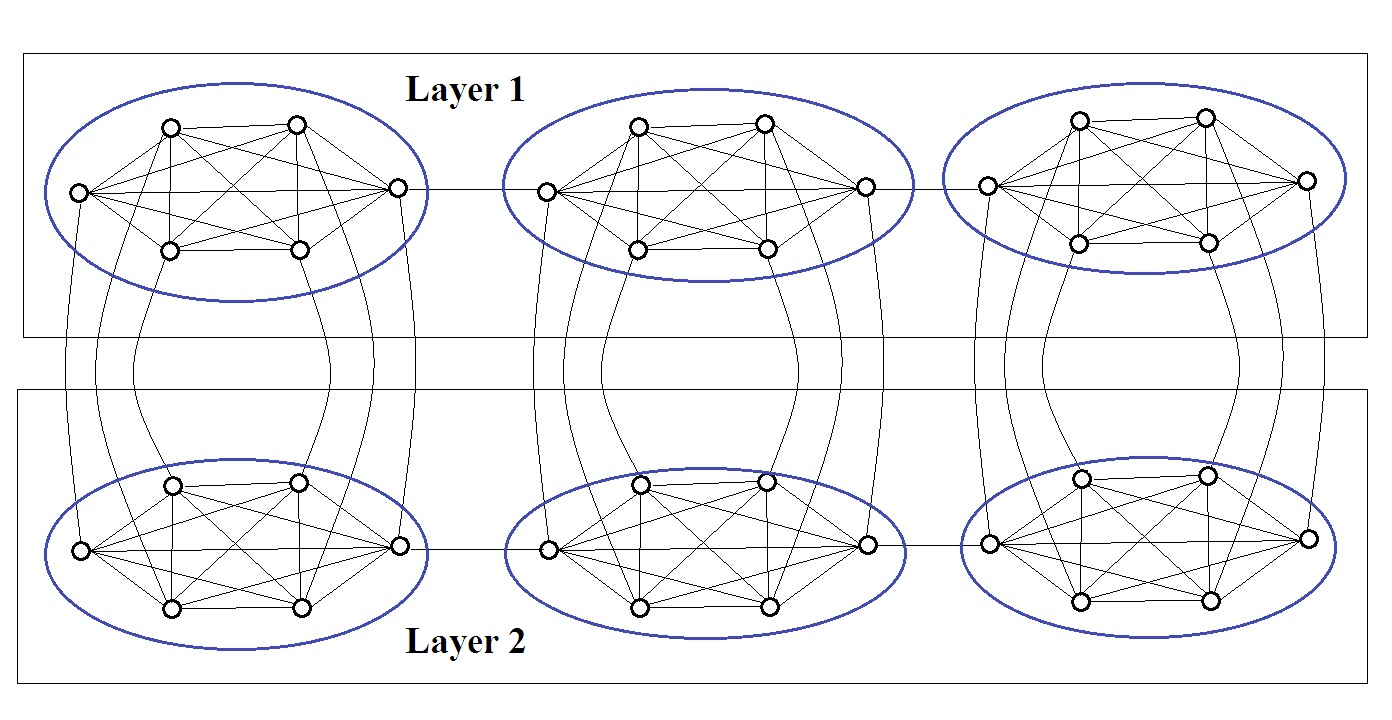
\includegraphics[angle=0,scale=.25]{./images/network0_2.jpg}}
% \end{center}
% \vspace{-0.22in}
% \caption{Network configuration with two different ground truth communities}
% \label{N0}
% \end{figure}



%Obviously, this modularity definition is not generic as it is defined for 2-layer networks only. 
The main deficiency of this definition comes from the fact that it checks the quality of a multilayer community 
by individually checking its 
single layer and bipartite components. It never checks how well the individual single layer components within each cross-layer community
are connected with each other.

For example, in Fig.~\ref{N0}, we show a two-layer network configuration with strong single layer modules (cliques of 100 nodes). 
There are same number of cliques (of same sizes) in both layers. Each clique in the top layer corresponds to exactly one clique in 
the bottom layer 
and there exists one-to-one coupling connections (total 300 coupling links) between the corresponding nodes.
We consider two different ground truth communities as shown in Fig.~\ref{N0} - one consisting of only single-layer communities 
(six in total), another 
consisting of only mixed communities (three in total).
If we gradually delete a fraction of coupling edges (randomly chosen), it is expected that the modularity corresponding 
to the multilayer ground truth would decrease and the modularity corresponding to single layer ground truth would 
increase. But, Fig.~\ref{mQ1} shows that 
none of this is actually captured by $mQ$. It throughout remains constant with coupling edge deletion. 
In case of multilayer communities it only decreases abruptly once all the coupling edges get deleted. 

\begin{figure}
\centering
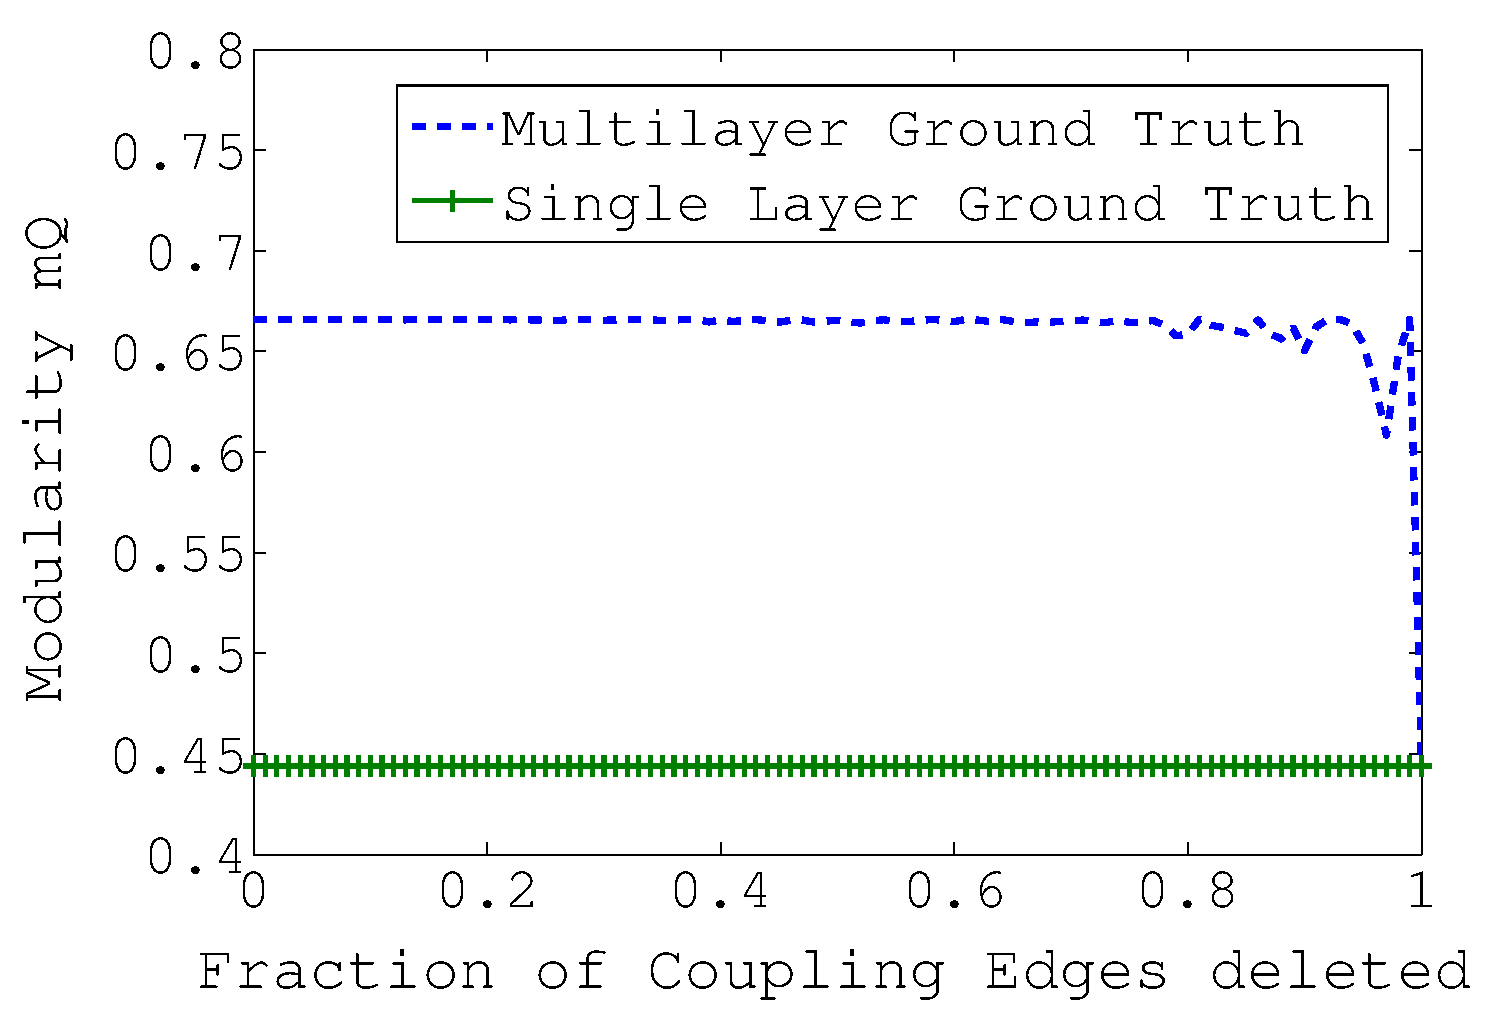
\includegraphics[width=2.5in]{./images/mQ_config1_2_100_5_no_ext_random_removal.pdf}
\vspace{-0.1in}
\caption{Change in mQ while deleting couplinng edges for both ground truth communities in Fig.~\ref{N0}}
\vspace{-0.1in}
\label{mQ1}
\end{figure}

The reason of this behaviour can be explained in the following way - in case of
single layer ground truth communities, the communities themselves do not include any coupling edge at all. So, in the calculation 
of modularity $mQ$, the coupling edges have no contribution and that is why $mQ$ remains constant even 
if more coupling edges get deleted.
On the other hand, for multilayer ground truth communities, each community has two single layer components and one coupling component.
The modularities of the single layer components do not change with coupling edge removal for the same reason stated above. 
But the bipartite modularity of the coupling component is expected to decrease with the deletion of coupling edges. 
Unfortunately, that does not happen. 
In our case, each coupling component is basically a set of parallel coupling edges.
When we remove the coupling edges, both numerator and denominator of the calculated bipartite modularity decreases (as there is no cross
community coupling edges) - essentially keeping
the total modularity sum almost constant.
% If there are E number of such edges in a multilayer community at any
% moment, the bipartite modularity of that component will 
% be $(E/(m*E)-(E*E)/(m*E)^2) = (1/m-1/m^2)$ where m is the number of multilayer communities ($m*E$ is the total number of coupling edges
% at this moment). 
So, the modularity of the coupling component of each community also becomes independent of the number of coupling edges present in the
network. This in turn makes the entire $mQ$ constant with respect to coupling edge deletion.
At the end when all the coupling edges get deleted, the bipartite modularity part of each community vanishes, resulting in a sudden drop in 
the total modularity.

In the next section, we propose our modularity metric which takes care of this limitations of $mQ$ by increasing its sensitivity about
how well the coupling links connect individual single layer components in each multilayer community.
% In Fig.~\ref{NN}, we show another network configuration with almost same configuration as Fig.~\ref{NN0} except that here 
% we have a strongly connected bipartite portion attached with each single layer clique. Similar to previous case,
% we consider two different ground truth communities as shown in Fig.~\ref{N01} and Fig.~\ref{N02}.
% If we gradually delete the coupling edges (except the ones in the bipartite clique part) one by one, 
% it is expected that the modularity corresponding to multilayer ground truth 
% should decrease and the modularity corresponding to single layer ground truth should increase. 
% Fig.~\ref{mQ2} shows that in this case also, the metric mQ is not sensitive to the quality of the multilayer communities.
% This happens because of the same reason as in the case of configuration 1. The modularities of single layer components of each 
% multilayer community do not get affected by the deletion of coupling edges. Only the bipartite modularity of the coupling portion 
% could have got affected. But unfortunately it doe not. Suppose, we have E number of coupling edges in a multilayer community at a 
% point of time other than the 5*5 dense bipartite portion. 
% Then the bipartite modularity of that coupling component of the community would 
% be $((E+25)/(m*(E+25))-((E+25)*(E+25))/(m*(E+25))^2) = (1/m-1/m^2)$ 
% where m is the number of multilayer communities ($m*(E+25)$ is the total number of coupling edges
% at this moment). So, here also, this factor is independent of the number of coupling edges present. 
% That is why the overall modularity of the multilayer communities does not change even if we delete coupling edges gradually.
% 
% In case of single layer ground truth communities, there is a difference from the result of configuration 1, due to the presence of 
% 5*5 strongly connected bipartite communities. As the total number of coupling edges (which is in the denominator 
% of the bipartite modularity definition) decrease at every step, the modularities of those three 5*5 communities improve. 
% The modularities of other six purely single layer 
% communities do not vary with coupling edge deletion. So, overall $mQ$ of the network increases with coupling edge deletion i.e.
% the metric is able to detect changes with respect to the single layer ground truth in case of configuration 2.
% 
% 
% 
% \begin{figure}
% \begin{center}
% \subfigure[Starting Configuration
% ]{\label{NN}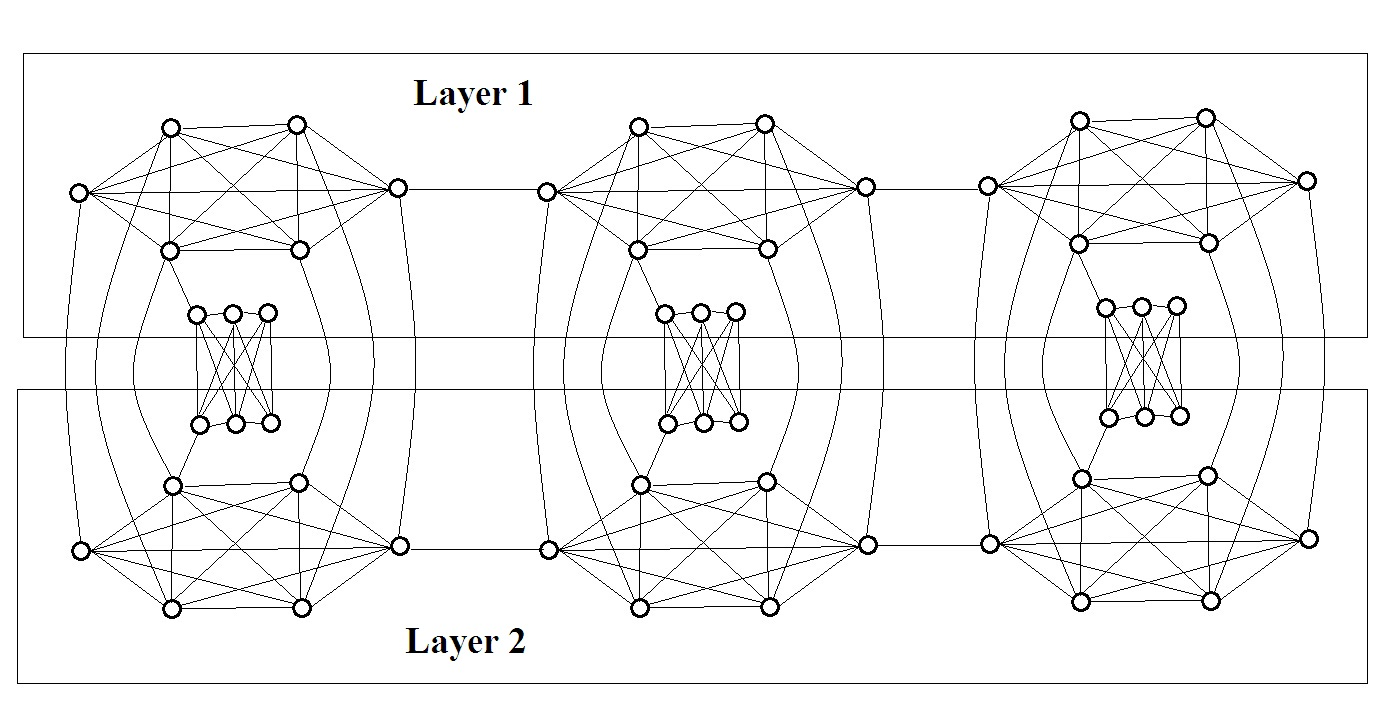
\includegraphics[angle=0,scale=.3]{./images/network.jpg}}
% \subfigure[Ground Truth multilayer communities
% ]{\label{N1}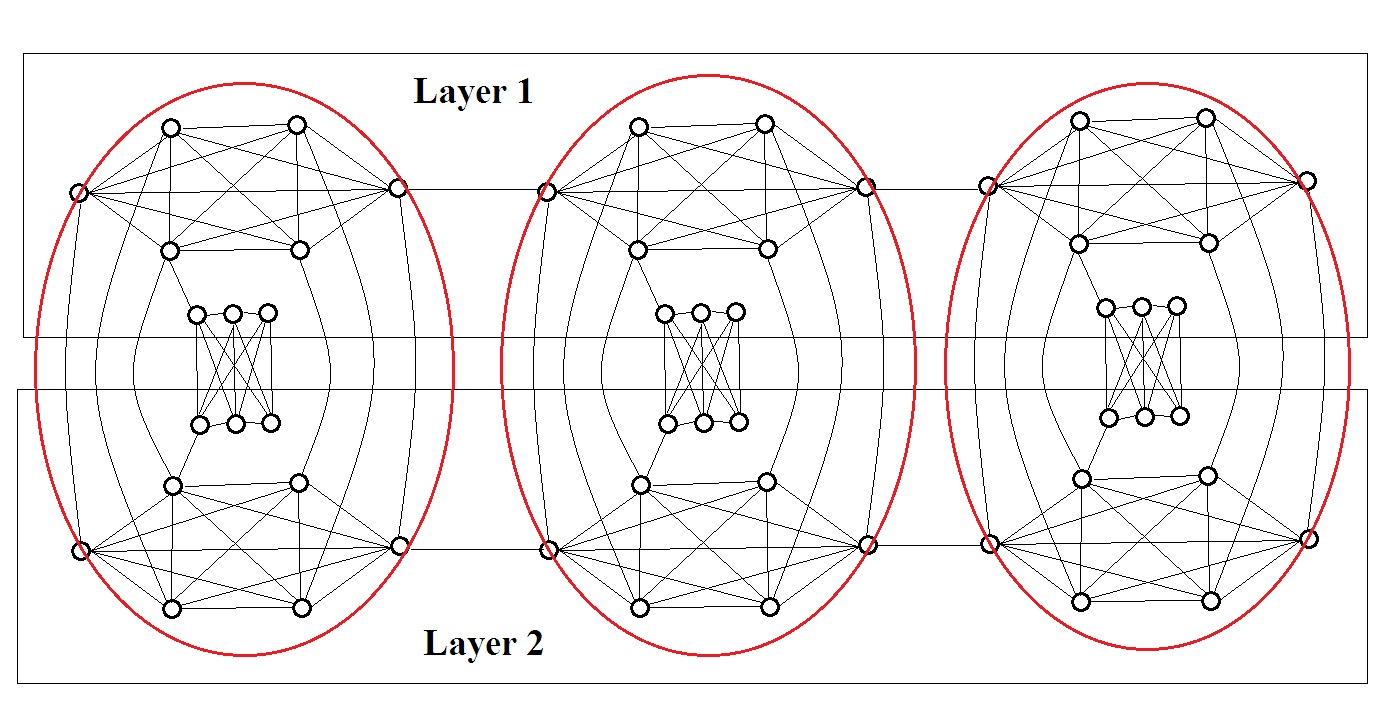
\includegraphics[angle=0,scale=.3]{./images/network1.jpg}}
% \subfigure[Ground Truth Single layer communities
% ]{\label{N2}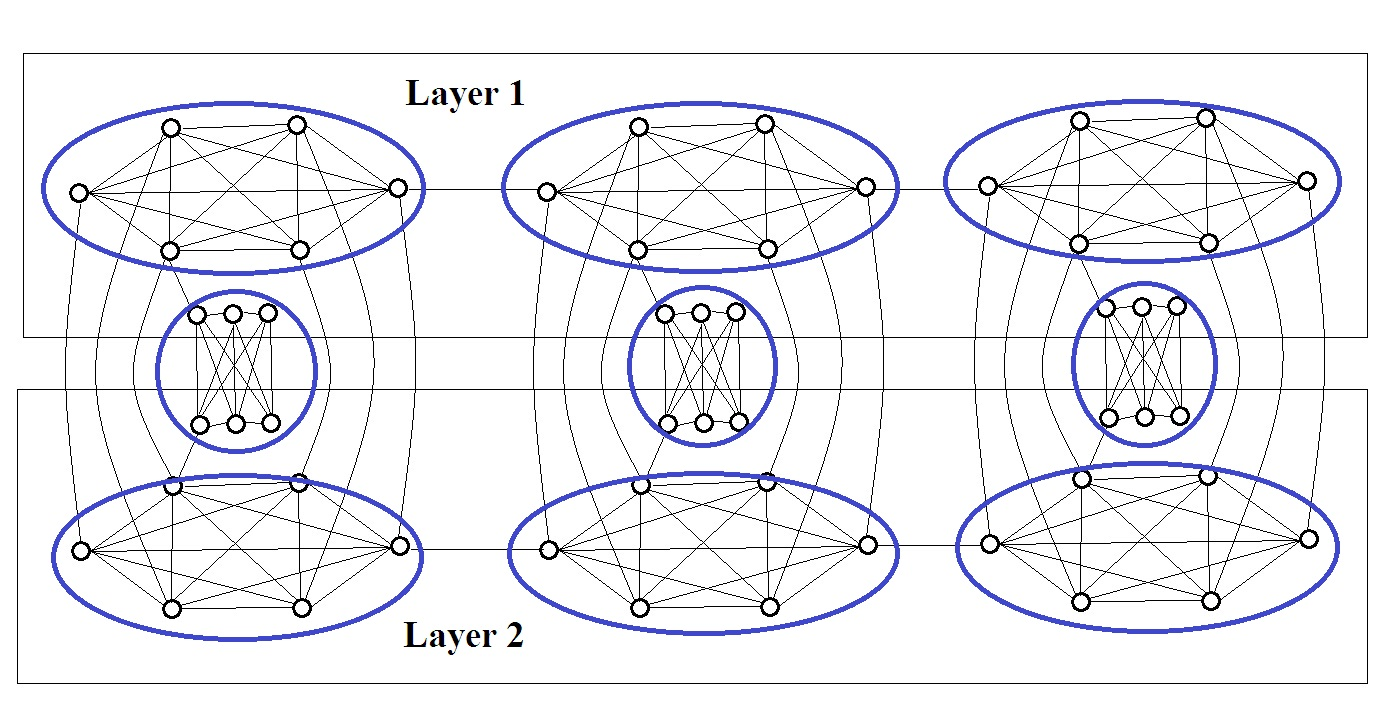
\includegraphics[angle=0,scale=.3]{./images/network2.jpg}}
% \end{center}
% \vspace{-0.22in}
% \caption{Network configuration 2 with two different ground truth communities}
% \label{N}
% \end{figure}
% 
% \begin{figure}
% \centering
% 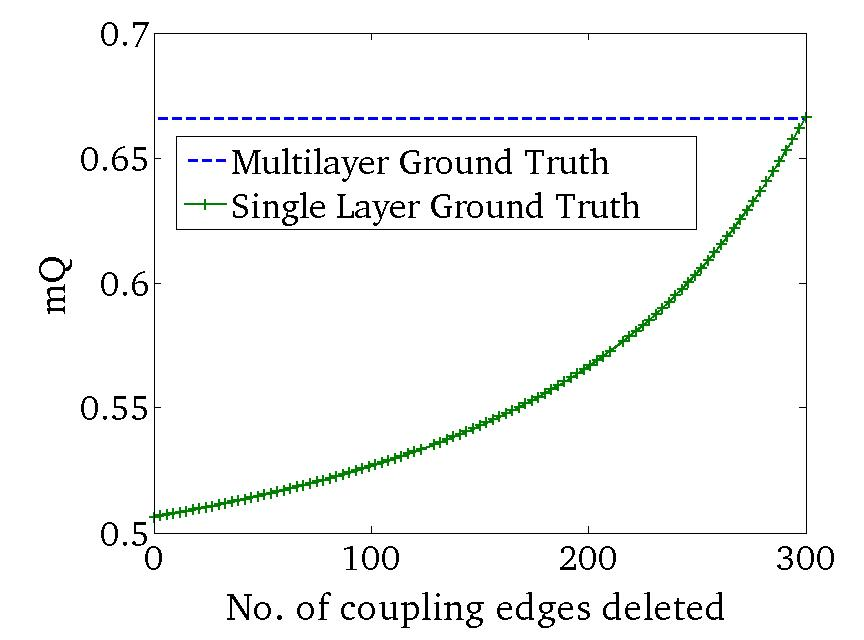
\includegraphics[width=2.5in]{./images/mQ_config1_2_100_5.jpg}
% \vspace{-0.1in}
% \caption{Change in mQ while deleting coupling edges for both ground truth communities in configuration 2}
% \vspace{-0.1in}
% \label{mQ2}
% \end{figure}
% 
% \textcolor{red}{[SP: We should try to generalize more on the limitation of $mQ$. To emphasize the superiority of our metric - 
% Is it enough to show that $mQ$ is not sensitive to a particular type of networks (as generic as possible) and 
% sensitive to other types of networks whereas our metric is sensitive to all types of networks?\\
% Can we get an idea from the configurations 1\& 2 here, about how to modify $Q_{adapt}$? We can also consider the weighted version of 
% $mQ$ with different weightages to single layer and cross-layer components.]
% }
